\documentclass{style/nseJournal}
\usepackage{graphicx}
\usepackage{amsmath}
\usepackage{amssymb}
\usepackage{hyperref}
\usepackage{booktabs}

\newcommand{\isotope}[2]{\ensuremath{^{#1}\mathrm{#2}}}

\newcommand{\sbin}{\langle \sigma \rangle}


\title{Variance Preservation for URR Probability Tables}
\correspondingEmail{golasa@rpi.edu}

\addAuthor{\correspondingAuthor{Alec Golas}}{1}
\addAuthor{Y. Danon}{1}
\addAuthor{A. Lewis}{2}
\addAuthor{D. Barry}{3}

% Affiliations
\addAffiliation{1}{Rensselaer Polytechnic Institute, Troy, NY, USA}
\addAffiliation{2}{Los Alamos National Laboratory, Los Alamos, NM, USA}
\addAffiliation{3}{Naval Nuclear Laboratory (Knowles Atomic site), West Milton, NY, USA}



\begin{document}
\titlePage

\begin{abstract}
Accurate treatment of resonance self-shielding in the Unresolved Resonance Region (URR) requires representing not only the infinitely-dilute mean cross section but also the variance associated with unresolved fluctuations. Probability tables are widely used to supply this fluctuation distribution; however, when the sampled-table mean differs from the evaluator mean used in transport, standard mean enforcement can inadvertently rescale the intended variance and bias self-shielding. Furthermore, when the evaluation's pointwise cross section (File~3) itself carries resonant structure---as in the ENDF/B-VIII.1 \isotope{235}{U} fission cross section---standard processing double counts the variance already present in File~3 and the full fluctuation variance encoded in the probability table. We derive a variance-preserving affine transformation that enforces the evaluator mean while retaining the physically sampled variance, and extend it to a per-reaction variance-budgeting methodology that partitions the total fluctuation variance between the File~3 and probability-table components. The variance decomposition is validated using a controlled \isotope{235}{U} transmission study, and the per-reaction implementation in NJOY/PURR is demonstrated for the ENDF/B-VIII.0 and VIII.1 evaluations. Integral benchmarks using the HEU-MET-INTERM-011 suite show a consistent $\sim$14~pcm reactivity shift from the mean-enforcement correction alone, corresponding to approximately 16\% of the total URR self-shielding reactivity worth.

\end{abstract}

%=============================================================================
\section{Introduction}
%=============================================================================

The energy-dependent structure of neutron cross sections is categorized into distinct regions. Between the Resolved Resonance Region (RRR) and the continuum region lies the Unresolved Resonance Region (URR), where cross sections possess resonance structure, but individual resonances cannot be resolved experimentally. URR evaluations are thus limited to average cross sections and average resonance parameters. This representation omits the large variance in the cross section's magnitude, which introduces a critical non-linear relationship between the average cross section and the average neutron transmission. This effect is known as resonance self-shielding.

The standard method to account for URR self-shielding in transport codes is the use of probability tables. These tables provide a discrete probability distribution of cross-section values, generated by statistically sampling many resonance ladders to reflect the underlying fluctuation content. For self-shielding to be physically consistent, the variance implied by the sampled resonance physics must be preserved when the probability table is applied in transport.

This paper identifies two distinct mechanisms by which that variance can be distorted in standard processing workflows. The first is an inadvertent variance scaling that arises when the probability-table mean differs from the evaluator's infinitely-dilute mean and a multiplicative normalization is used to enforce consistency. The second is a variance double-counting problem that arises when the evaluation's pointwise File~3 cross section carries resonant structure while the probability table continues to represent the full compound-nucleus fluctuation variance.

Both problems have become practically urgent with recent evaluation changes. In the transition from ENDF/B-VIII.0 to ENDF/B-VIII.1~\cite{endf-8.0,endf-8.1}, significant resonant structure was introduced into the \isotope{235}{U} fission cross section within the URR, making the double-counting problem newly relevant for a major fissile isotope. This paper derives variance-preserving corrections for both problems, implements them in the NJOY processing code, and validates the methodology using controlled transmission tests and integral criticality benchmarks.

%=============================================================================
\section{Background}
\label{sec:background}
%=============================================================================

%-----------------------------------------------------------------------------
\subsection{Role of Variance in URR Self-Shielding}
\label{ssec:variance-role}
%-----------------------------------------------------------------------------

In the Unresolved Resonance Region (URR), the nucleus possesses a fixed resonance ladder, but individual resonances cannot be resolved experimentally due to limited resolution and the high density of levels. Consequently, URR evaluations specify \emph{average} resonance parameters together with an assumed statistical model (e.g., level spacings drawn from a Wigner distribution, widths from a Porter--Thomas distribution) representing the ensemble of resonance ladders consistent with those averages. These average parameters are then used to generate distributions of cross sections from which realizations can be sampled in transport codes.

The connection between resonance self-shielding and variance follows from the nonlinearity of neutron transmission. For a path length $n$, the transmission involves $\exp(-n\sigma)$, and the transmission of the average cross-section does not equal the average transmission, or
\begin{equation}
\left\langle \exp\!\left(-n\sigma\right) \right\rangle \neq \exp\!\left(-n\left\langle \sigma \right\rangle\right),
\end{equation}
where $\langle\cdot\rangle$ denotes some energy-averaged quantity. Then separating out the transmission of the mean cross-section component, $\exp{\left(-n\langle\sigma\rangle\right)}$:
\begin{equation}
\langle T\rangle \;=\; \left\langle e^{-n\sigma(E)}\right\rangle
\;=\; \left\langle e^{-n\left[ \sigma(E) + \langle \sigma \rangle - \langle \sigma \rangle \right]} \right\rangle
\;=\; e^{-n\langle\sigma\rangle}\left\langle e^{-n\left[\sigma(E) - \langle \sigma \rangle \right]}\right\rangle.
\end{equation}
Expanding $\left\langle e^{-n\left[\sigma(E) - \langle \sigma \rangle \right]}\right\rangle$ as a Taylor series gives
\begin{equation}
\left\langle e^{-n\left[\sigma(E) - \langle \sigma \rangle \right]}\right\rangle
= 1 - n\left\langle \left[\sigma(E) - \langle \sigma \rangle \right] \right\rangle + \frac{n^2}{2}\left\langle \left[\sigma(E) - \langle \sigma \rangle \right]^2 \right\rangle
\end{equation}
and therefore
\begin{equation}
\left\langle e^{-n\sigma}\right\rangle
\;\approx\;
e^{-n\langle\sigma\rangle}\left[\,1+\frac{n^2}{2}\,\mathrm{Var}(\sigma)\,\right]
\label{eq:transmission_variance_link}
\end{equation}
\autoref{eq:transmission_variance_link} makes the key point explicit: even when two URR representations share the same bin-averaged mean $\langle\sigma\rangle$, the cross-section variance changes $\langle T\rangle$ independently of the mean cross-section. Consequently, reproducing URR self-shielding requires that the transport code receive a distribution with both the correct bin-averaged mean (supplied by the evaluator's File~3 cross section) and the correct fluctuation variance (determined by the statistical model of File~2 average resonance parameters).

%-----------------------------------------------------------------------------
\subsection{Variance Independence from the Infinitely Dilute Average Cross-Section}
\label{ssec:variance-independence}
%-----------------------------------------------------------------------------

The core result of KKM theory \cite{Kawai1973} decomposes the scattering matrix into a smooth component and a fluctuating component:
\begin{equation}
S_{cc'}(E) = S_{cc'}^{\text{opt}}(E) + S_{cc'}^{\text{fl}}(E),
\end{equation}
where the energy average over the bin satisfies
\begin{equation}
\langle S^{\text{opt}}(E)\rangle_I = S^{\text{opt}}(E), \qquad \langle S^{\text{fl}}(E)\rangle_I = 0.
\end{equation}
The corresponding cross section similarly separates into optical and fluctuation components\cite{Carlson_2014}:
\begin{equation}
\sigma_{cc'} = \sigma_{cc'}^{\text{opt}} + \sigma_{cc'}^{\text{fl}},
\end{equation}
where the fluctuation cross section is given by
\begin{equation}
\sigma_{cc'}^{\text{fl}} = \left\langle \left| S_{cc'}^{\text{fl}} \right|^2 \right\rangle.
\end{equation}
The within-bin variance is then
\begin{equation}
V = \left\langle \left(\sigma_{cc'} - \langle \sigma_{cc'} \rangle \right)^2 \right\rangle = \left\langle \left(\sigma_{cc'} - \sigma_{cc'}^{\text{opt}} \right)^2 \right\rangle = \left\langle \left(\sigma_{cc'}^{\text{fl}}\right)^2 \right\rangle,
\end{equation}
which depends only on the fluctuating component and is independent of the bin mean $\sigma_{cc'}^{\text{opt}}$.

This shows that the fluctuations of the cross-section is independent of $\langle \sigma \rangle$, and one cannot derive $\mathrm{Var}(\sigma)$ from $\langle \sigma \rangle$ or vice versa. Therefore, adding additional components (smooth intermediate structure, direct reactions, increasing the potential scattering term, etc.) should have no impact on the variance of the cross-section. This independence is the theoretical foundation for the variance-budgeting approach developed in \autoref{sec:theory}: because the fluctuation variance $V$ is determined solely by the compound-nucleus statistical properties (File~2 average resonance parameters), it is independent of whatever smooth structure the evaluator chooses to include in the mean cross section (File~3), and can therefore be partitioned between these two representations without loss of generality.

%-----------------------------------------------------------------------------
\subsection{Probability-Table Representation of URR Fluctuations}
\label{ssec:ptable-background}
%-----------------------------------------------------------------------------

Probability tables provide a discrete representation of the within-bin distribution of cross sections\cite{Levitt1972Probability}. In an energy bin, a p-table supplies cross-section values $\{\sigma_j\}$ with probabilities $\{P_j\}$,
\begin{equation}
\sum_j P_j = 1.
\end{equation}
Two summary quantities are the probability-table distribution mean and variance,
\begin{equation}
\mu \equiv \sum_j P_j \sigma_j,
\label{eq:mu_def}
\end{equation}
\begin{equation}
V \equiv \sum_j P_j(\sigma_j-\mu)^2.
\label{eq:V_def}
\end{equation}
Here $\mu$ denotes the expected value under the discrete distribution $\{P_j, \sigma_j\}$ produced by the ladder sampling, not a population parameter. Separately, the evaluation provides the target infinitely-dilute bin mean cross section, denoted here by $\sbin$ and stored in File~3 of the ENDF data.
A physically consistent URR treatment should therefore satisfy two conditions simultaneously:
(i) the distribution used in transport must reproduce $\sbin$ as its mean, and
(ii) it must preserve the physically sampled variance $V$ implied by the ladder ensemble.

The following two subsections describe how each of these conditions can be violated in standard processing workflows.

%-----------------------------------------------------------------------------
\subsection{Problem~1: Mean Enforcement via Multiplicative Scaling}
\label{ssec:lssf_flaw}
%-----------------------------------------------------------------------------

In practice, differences in evaluation and processing formalisms (e.g., Reich--Moore versus SLBW approximations), together with URR processing details, can produce noticeable discrepancies between the probability-table distribution mean $\mu$ and the evaluator-supplied mean $\sbin$ \cite{Cullen2010ENDF,Sublet2009}. A common practice to enforce mean consistency is to store probability tables as dimensionless factors (e.g., \texttt{LSSF=1} in ENDF-6 format terminology \cite{endf-manual}):
\begin{equation}
f_j \equiv \frac{\sigma_j}{\mu},
\label{eq:ptable-orig-factor}
\end{equation}
so that $\sum_j P_j f_j = 1$.
During transport, the cross section is reconstructed as
\begin{equation}
\sigma_j^{(\times)} = f_j\,\sbin,
\label{eq:sigma_times}
\end{equation}
which guarantees the evaluated mean is recovered:
\begin{equation}
\sum_j P_j \sigma_j^{(\times)} = \sbin.
\end{equation}

However, \autoref{eq:sigma_times} scales the \emph{entire} sampled distribution by the factor $\sbin/\mu$. Since $\mathrm{Var}(aX)=a^2\mathrm{Var}(X)$, the variance seen by the transport code becomes
\begin{equation}
\mathrm{Var}\!\left(\sigma^{(\times)}\right) = \left(\frac{\sbin}{\mu}\right)^2 V.
\label{eq:var_scaling}
\end{equation}
Thus, whenever $\sbin \neq \mu$, the variance that was physically implied by the sampled ladder ensemble is artificially inflated or suppressed. This effect is illustrated in \autoref{fig:dist-example} for \isotope{235}{U} at 2.4~keV, where the standard factor normalization visibly broadens the cross-section distribution. Because URR self-shielding is driven by this variance through the nonlinearity of transport observables, this normalization choice produces a systematic bias in self-shielding while enforcing the correct bin mean. The resulting bias in self-shielded transmission is shown in \autoref{fig:fig2}.

\begin{figure}[htbp]
\centering
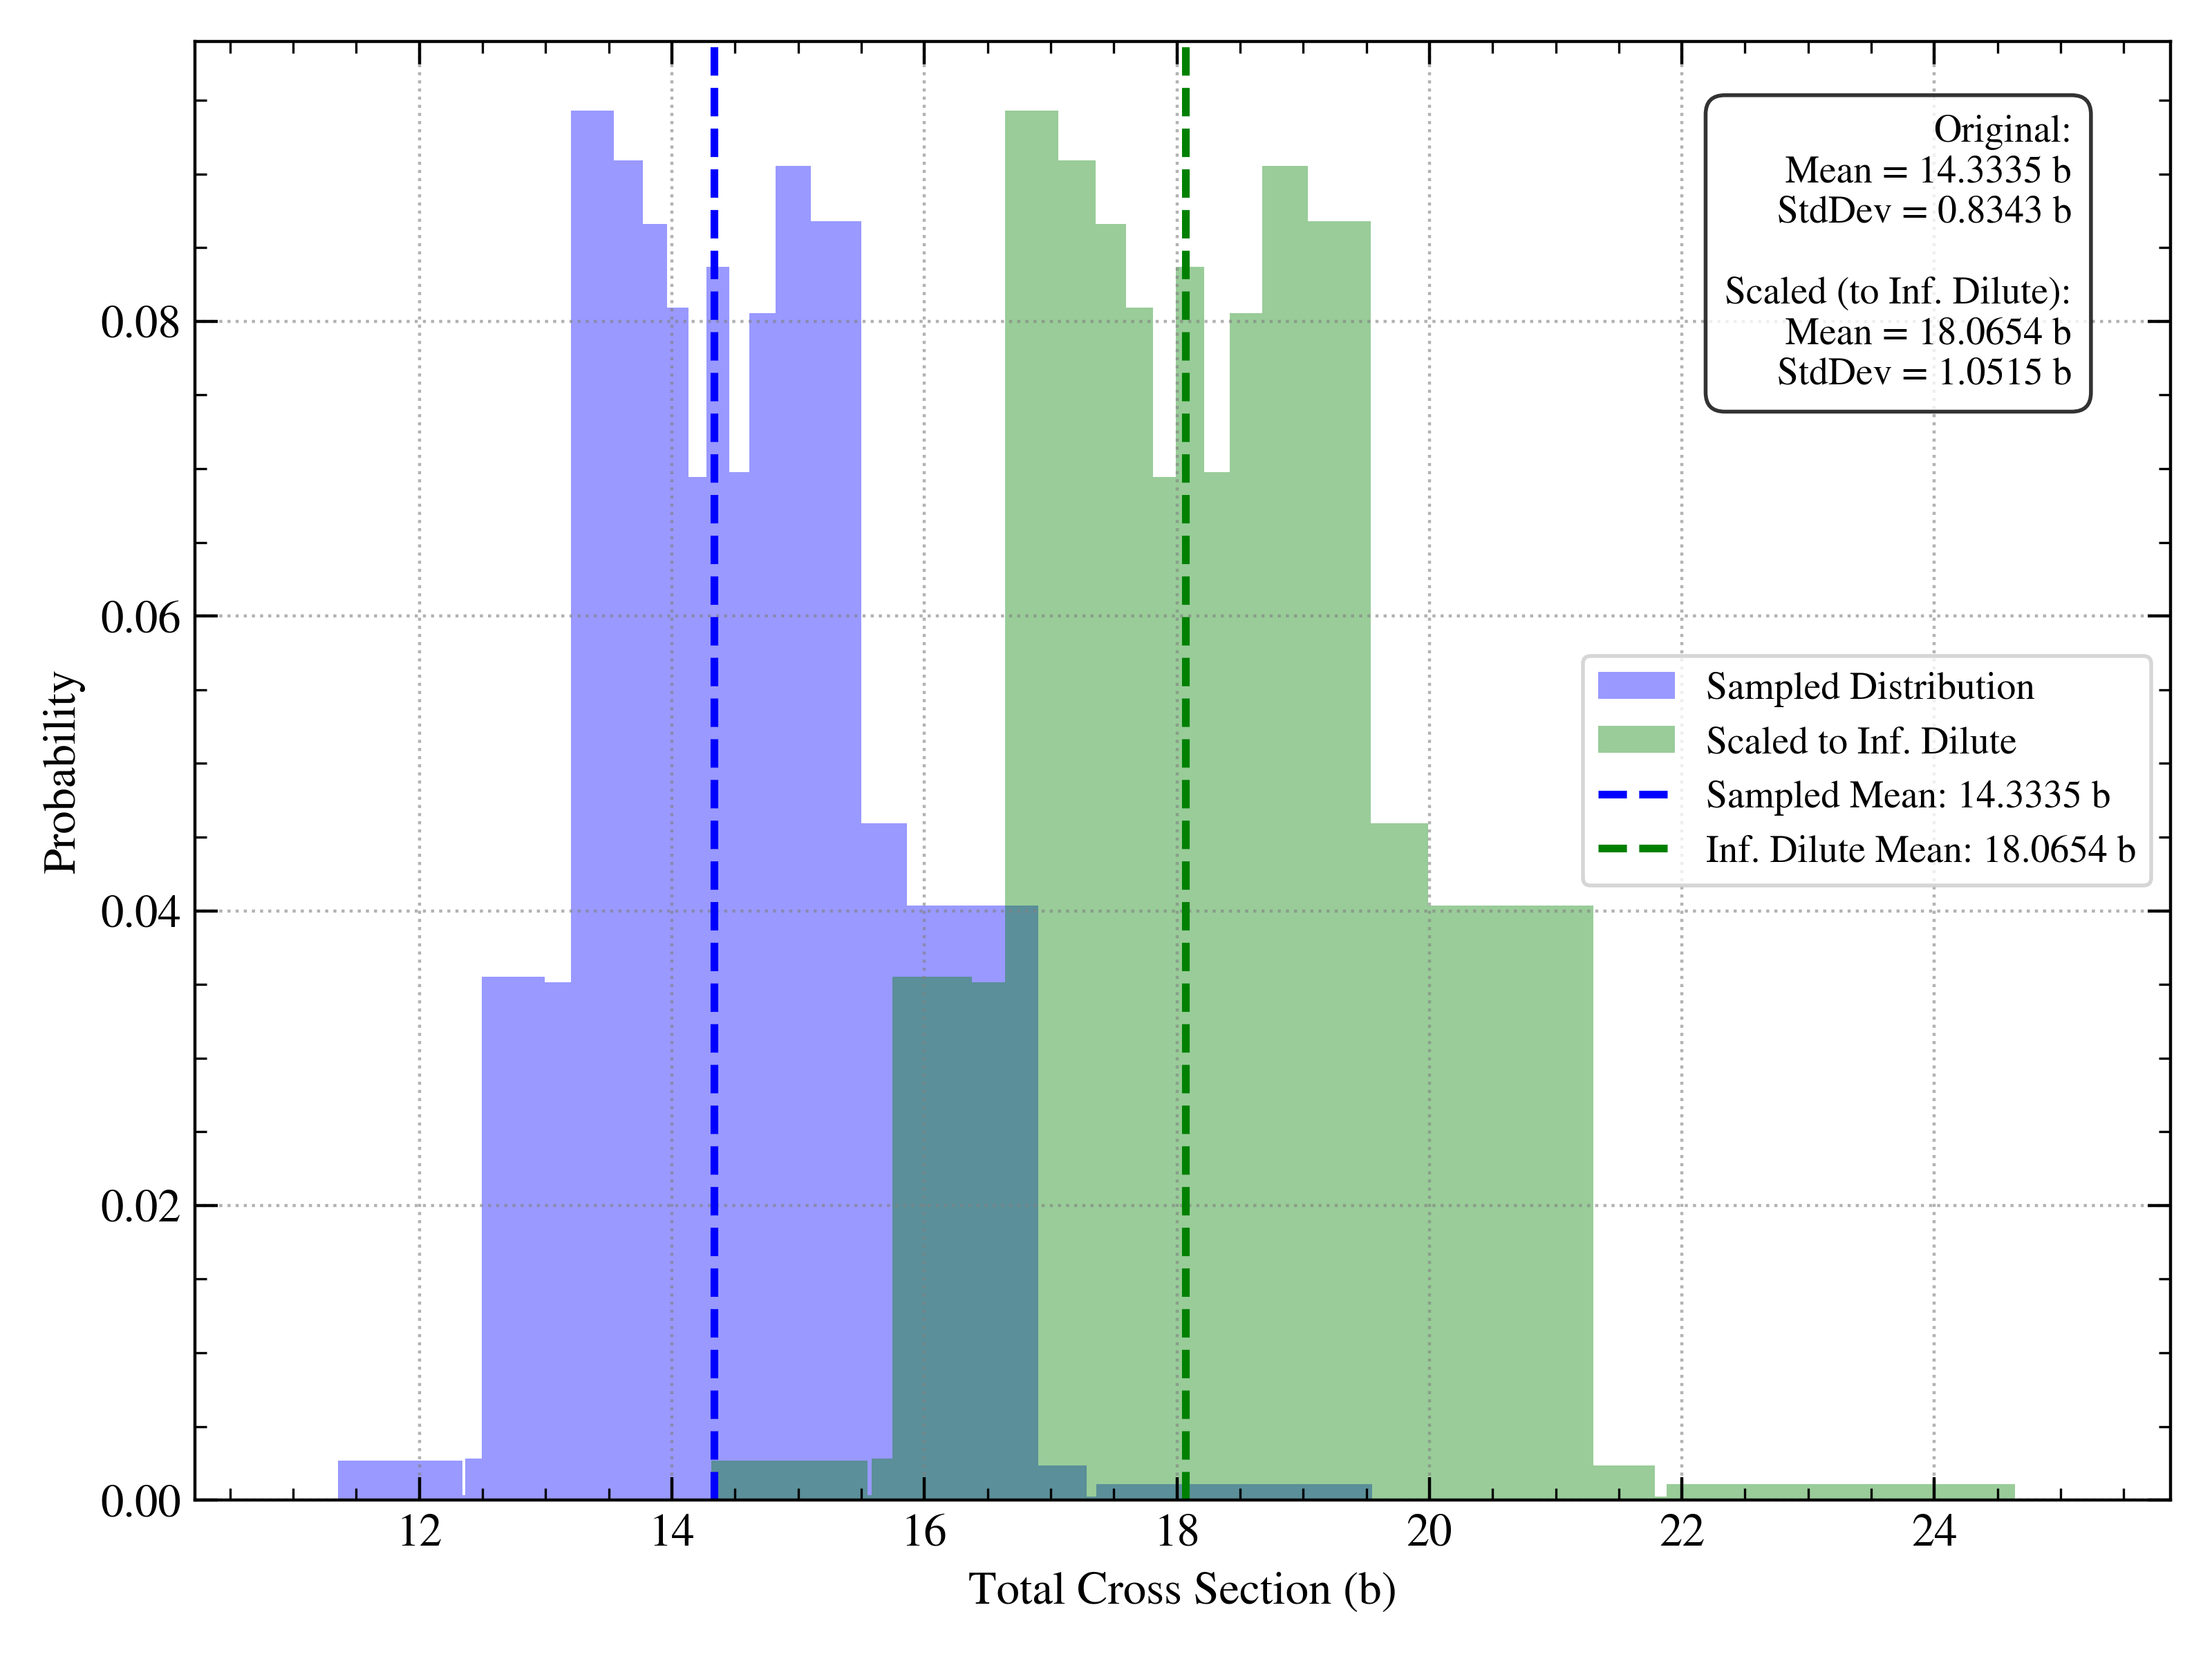
\includegraphics[width=0.95\linewidth]{figures/dist_compare_E_2.400e+04eV.png}
\caption{Comparison of the original sampled p-table distribution for \isotope{235}{U} at 2.4~keV and the distribution obtained by standard factor normalization using the evaluator mean. The latter scales the distribution by $\sbin/\mu$ (here, $>1$), broadening the distribution and inflating the variance (cf.\ \autoref{eq:var_scaling}).}
\label{fig:dist-example}
\end{figure}

\begin{figure}[htbp]
\centering
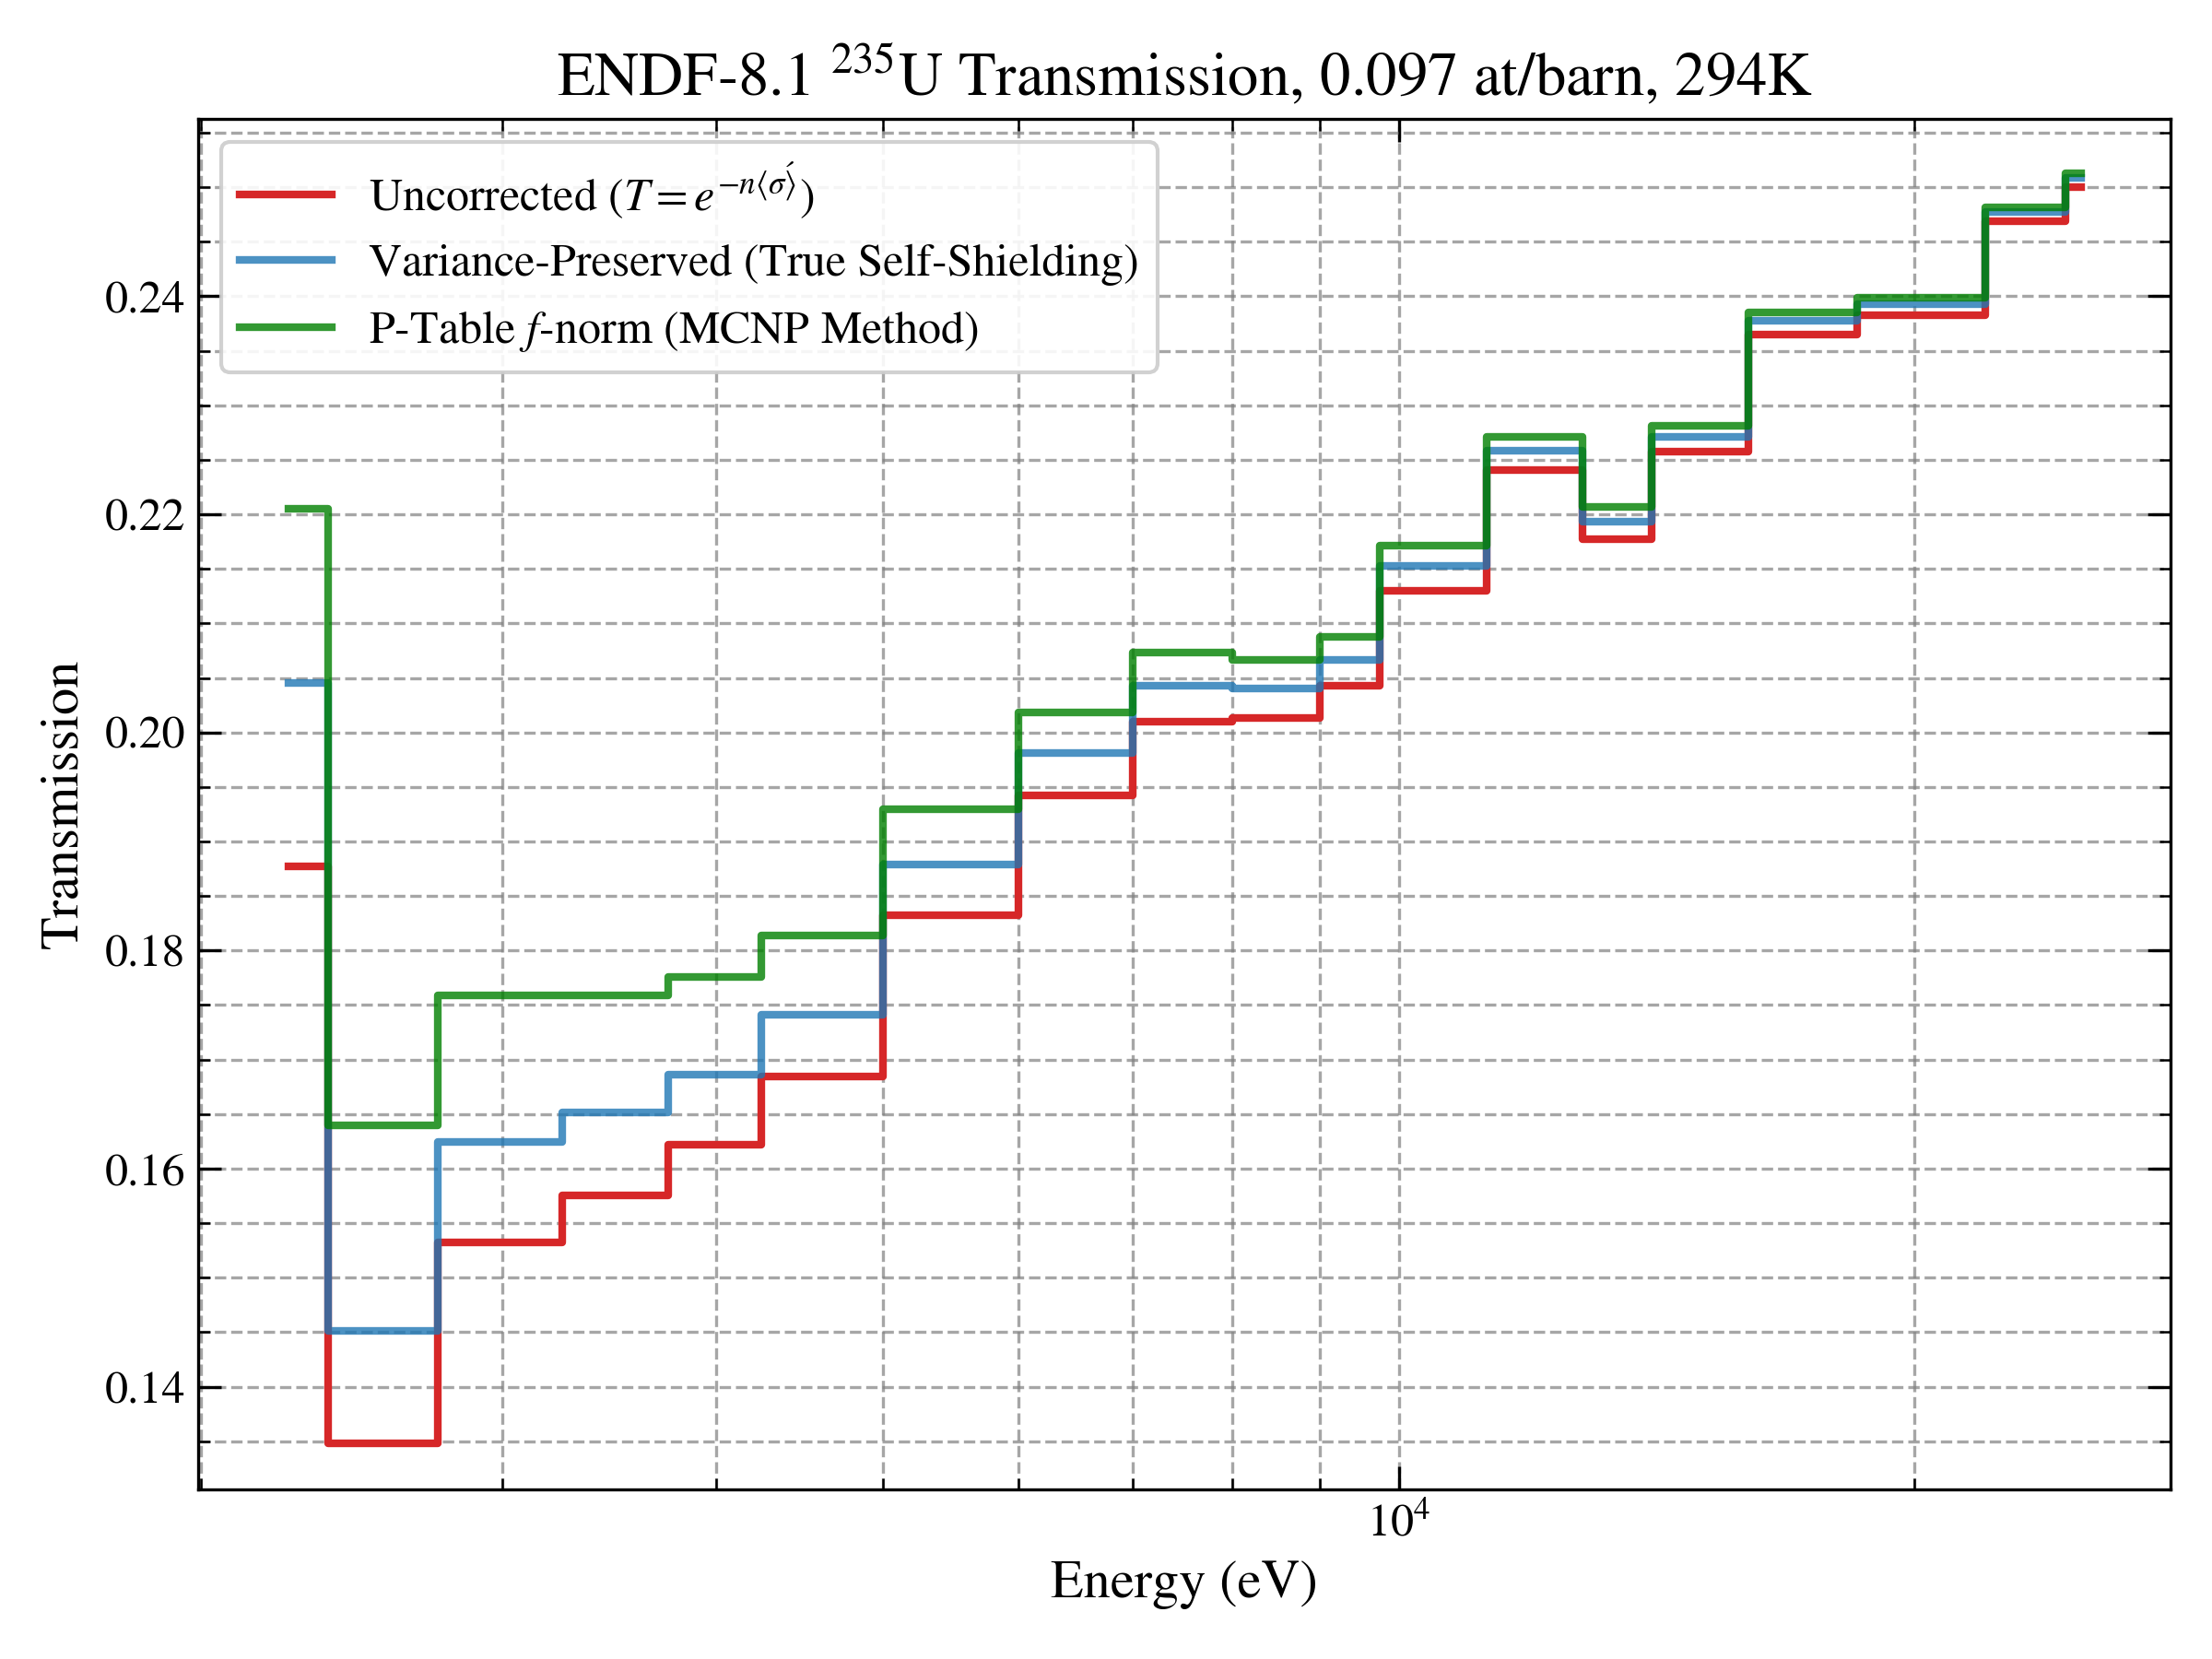
\includegraphics[width=0.95\linewidth]{figures/u235_transmission_plot_demo.png}
\caption{Comparison of self-shielded transmission calculations for \isotope{235}{U}. The standard factor-normalized p-table method deviates from the variance-preserving result due to inadvertent variance scaling.}
\label{fig:fig2}
\end{figure}

%-----------------------------------------------------------------------------
\subsection{Problem~2: Variance Double Counting from File~3 Structure}
\label{ssec:double-counting-problem}
%-----------------------------------------------------------------------------

The multiplicative scaling problem described above distorts the variance when $\sbin \neq \mu$, but even when these means agree, a second source of variance distortion can arise whenever the File~3 pointwise cross section $\sigma_3(E)$ carries resonant structure within a probability-table bin.

Under the standard \texttt{LSSF=1} processing workflow, probability tables are generated from the evaluation's average resonance parameters and represent the full compound-nucleus fluctuation variance $V$. Separately, the File~3 cross section provides the pointwise mean $\sigma_3(E)$ used in transport. If $\sigma_3(E)$ is smooth within each bin, it contributes negligible within-bin variance and the probability table supplies all the fluctuation content---as intended. However, if $\sigma_3(E)$ carries significant resonant structure, the transport code effectively sees \emph{two} sources of within-bin variance: the fluctuations in $\sigma_3(E)$ itself (characterized by $V_3$) and the full p-table fluctuation variance $V$. The result is a total effective variance of $V_3 + V$, which exceeds the intended compound-nucleus variance $V$ and produces excess self-shielding.

\subsubsection{Motivating Example: \isotope{235}{U} Fission in ENDF/B-VIII.1}
\label{sssec:u235-evaluation-change}

The transition from ENDF/B-VIII.0~\cite{endf-8.0} to ENDF/B-VIII.1~\cite{endf-8.1} makes this problem concrete. Both evaluations draw on the same experimental fission cross-section dataset~\cite{WestonTodd1992}, but differ in how that data is incorporated into the File~3 pointwise cross section. ENDF/B-VIII.0 uses a heavily smoothed representation, retaining only modest within-bin structure ($V_{3,\text{fis}}$ up to $\sim$0.8~b$^2$ in the lowest-energy bins, decreasing rapidly with energy). ENDF/B-VIII.1 retains substantially more of the measured resonant structure, producing within-bin fission variance roughly an order of magnitude larger ($V_{3,\text{fis}}$ up to $\sim$2.5~b$^2$).

\autoref{fig:u235-fission-comparison} compares the pointwise fission cross sections across the URR for the two evaluations. \autoref{fig:v3-fission} shows the within-bin File~3 fission variance $V_{3,\text{fis}}$ at each PURR grid point. Elastic and capture cross sections are essentially identical between the two evaluations and contribute negligible $V_3$ in both cases (\autoref{fig:v3-elastic-capture}).

\begin{figure}[htbp]
\centering
%\includegraphics[width=0.95\linewidth]{figures/fig_u235_fission_comparison.pdf}
\caption{\isotope{235}{U} fission cross section in the URR for ENDF/B-VIII.0 and ENDF/B-VIII.1, both derived from the Weston \& Todd~\cite{WestonTodd1992} measurement but with different degrees of smoothing.}
\label{fig:u235-fission-comparison}
\end{figure}

\begin{figure}[htbp]
\centering
%\includegraphics[width=0.95\linewidth]{figures/fig_v3_fission.pdf}
\caption{Within-bin File~3 fission variance $V_{3,\text{fis}}$ at each PURR energy grid point. The VIII.1 evaluation carries roughly an order of magnitude more fission variance than VIII.0.}
\label{fig:v3-fission}
\end{figure}

Under the standard processing workflow, the probability tables for both evaluations are generated from the same average resonance parameters using PURR, and therefore represent the same full compound-nucleus fluctuation variance $V$. When the File~3 fission cross section was heavily smoothed (VIII.0), the standard approach introduced only a small double-counting bias. With the increased fission structure in VIII.1, the File~3 contribution $V_{3,\text{fis}}$ becomes a significant fraction of the total variance, but the p-table factors are not adjusted to account for the variance already present in File~3. The result is substantial variance double counting for the fission channel.

The two problems are related: both arise from the probability-table factor format failing to account for information outside the table itself. Problem~1 ignores the discrepancy between $\mu$ and $\sbin$; Problem~2 ignores the within-bin structure of $\sigma_3(E)$. The variance-preserving methodology derived in the next section addresses both through a unified affine transformation framework.

%=============================================================================
\section{Variance-Preserving Methodology and Implementation}
\label{sec:theory}
%=============================================================================

This section derives the variance-preserving transformations and describes their implementation in the NJOY/PURR processing code.

%-----------------------------------------------------------------------------
\subsection{Mean Correction with Variance Preservation}
\label{ssec:var-pres}
%-----------------------------------------------------------------------------

Given a sampled probability-table distribution $\{\sigma_j,P_j\}$ with mean $\mu$ and variance $V$, the goal is to determine a transformed set $\{\sigma'_j\}$ such that
\begin{equation}
\sum_j P_j \sigma'_j = \sbin,
\label{eq:mean_req}
\end{equation}
and
\begin{equation}
\sum_j P_j(\sigma'_j-\sbin)^2 = V.
\label{eq:var_req}
\end{equation}

Variance is invariant under additive shifts. Therefore, the minimal correction that enforces \autoref{eq:mean_req} while preserving \autoref{eq:var_req} is
\begin{equation}
\sigma'_j = \sigma_j + \Delta,
\label{eq:affine_shift}
\end{equation}
with
\begin{equation}
\Delta = \sbin-\mu.
\label{eq:Delta_def}
\end{equation}
This guarantees the transformed distribution has mean $\sbin$ and retains the original sampled variance $V$.

If factors are preferred for storage, the equivalent corrected factors are
\begin{equation}
f'_j \equiv \frac{\sigma'_j}{\sbin}
= \frac{\sigma_j + (\sbin-\mu)}{\sbin},
\label{eq:fprime_shift}
\end{equation}
which still satisfies $\sum_j P_j f'_j = 1$.

%-----------------------------------------------------------------------------
\subsection{Variance Budget with Within-Bin Structure}
\label{ssec:double-dipping}
%-----------------------------------------------------------------------------

The correction above assumes the entire within-bin variance relevant to self-shielding should be represented by the probability table. In some applications, one may wish to retain a fluctuating pointwise cross section $\sigma_3(E)$ (so named because this quantity is stored in File~3 of the ENDF data structure) within the bin while also representing additional unresolved fluctuations via probability-table sampling. In that case, variance can be double counted unless a variance budget is enforced.

Let $V$ continue to denote the total variance implied by the sampled ladder ensemble, as defined in \autoref{eq:V_def}. Let $V_3$ be the intra-bin variance already present in $\sigma_3(E)$. Now the target is a probability-table contribution $V_{\mathrm{PT}}$ satisfying
\begin{equation}
V = V_{\mathrm{PT}} + V_3,
\label{eq:var_split}
\end{equation}
neglecting a covariance term between the two components (discussed below). Therefore,
\begin{equation}
V_{\mathrm{PT}} = V - V_3.
\label{eq:VPT_def}
\end{equation}

This is resolved by performing an affine transform of the sampled distribution:
\begin{equation}
\sigma'_j = a\,\sigma_j + b.
\label{eq:affine_general}
\end{equation}
Because adding $b$ does not affect variance,
\begin{equation}
\mathrm{Var}(\sigma') = a^2 V.
\end{equation}
To enforce $\mathrm{Var}(\sigma')=V_{\mathrm{PT}}$, we require
\begin{equation}
a = \sqrt{1-\frac{V_3}{V}}.
\label{eq:a_def}
\end{equation}
The constant $b$ is set by enforcing the correct mean:
\begin{equation}
\sum_j P_j\sigma'_j = a\mu + b = \sbin
\quad\Rightarrow\quad
b = \sbin-a\mu.
\label{eq:b_def}
\end{equation}
Combining \autoref{eq:a_def}--\autoref{eq:b_def}, the variance-budgeted distribution is
\begin{equation}
\sigma'_j = \sbin + a(\sigma_j-\mu),
\qquad
a=\sqrt{1-\frac{V_3}{V}}.
\label{eq:sigma_prime_budget}
\end{equation}
In factor form,
\begin{equation}
f'_j = \frac{\sigma'_j}{\sbin}
= 1 + \frac{a}{\sbin}(\sigma_j-\mu).
\label{eq:fprime_budget}
\end{equation}

\autoref{eq:var_split} neglects the covariance between the unresolved component and $\sigma_3(E)$. In practice, estimating such a covariance requires attributing which structures in $\sigma_3$ correspond to structures in the ladder ensemble, information that is generally inaccessible in the unresolved regime. The variance-budgeting form above is therefore intended as a practical, controllable approximation.

Note that \autoref{eq:sigma_prime_budget} subsumes the pure mean-shift correction of \autoref{eq:affine_shift}--\autoref{eq:Delta_def} as the limiting case $V_3 = 0$ (i.e., $a = 1$). The two problems identified in \autoref{sec:background} are thus addressed by a single affine framework, with $a$ controlling the degree of variance reduction.

%-----------------------------------------------------------------------------
\subsection{Implementation in NJOY/PURR}
\label{ssec:njoy-implementation}
%-----------------------------------------------------------------------------

The variance-budgeting methodology is implemented in the PURR module of the NJOY nuclear data processing code~\cite{njoy}. Two modifications are required: computing the within-bin File~3 variance $V_3$ for each reaction at each probability-table energy grid point, and applying the per-reaction scaling parameter $a$ during factor generation.

\subsubsection{Computing Within-Bin File~3 Variance}
\label{sssec:compute-v3}

The probability-table energy grid $\{E_1, E_2, \ldots, E_N\}$ defines $N$ grid points at which PURR generates probability tables via statistical ladder sampling. The within-bin variance $V_3$ must be evaluated at each of these grid points and for each reaction channel independently (total, elastic, fission, capture), since different reactions may have very different degrees of pointwise structure. For \isotope{235}{U}, for example, the total cross section is essentially smooth in the URR ($V_3\approx 0$), while the fission cross section exhibits significant resonant structure ($V_3 > 0$).

For each grid point $E_i$, the relevant energy window is defined using geometric midpoints between adjacent grid points:
\begin{equation}
E_{i-\frac{1}{2}} = \sqrt{E_{i-1}\,E_i}, \qquad E_{i+\frac{1}{2}} = \sqrt{E_i\,E_{i+1}}.
\label{eq:half-interval}
\end{equation}
The use of geometric (rather than arithmetic) midpoints is appropriate because the URR grid points are approximately logarithmically spaced. The within-bin variance is then computed by densely sampling the File~3 cross section at $M$ uniformly spaced sub-points within $[E_{i-1/2},\,E_{i+1/2}]$:
\begin{equation}
V_{3,r}(E_i) = \frac{1}{M}\sum_{m=1}^{M}\sigma_{3,r}^2(E_m) - \left(\frac{1}{M}\sum_{m=1}^{M}\sigma_{3,r}(E_m)\right)^2,
\label{eq:v3-computation}
\end{equation}
where $\sigma_{3,r}(E_m)$ is the File~3 cross section for reaction $r$ at energy $E_m$ obtained via the standard ENDF interpolation law. The current implementation uses $M=200$, which provides adequate resolution for cross sections with resonant structure comparable to or broader than the average level spacing in the URR.

At the URR boundaries, one-sided intervals are used:
\begin{equation}
\text{First point:}\quad [E_1,\; E_{3/2}], \qquad \text{Last point:}\quad [E_{N-\frac{1}{2}},\; E_N].
\end{equation}
This avoids extrapolation outside the URR while still providing a local variance estimate at the boundary grid points. In practice, the first grid point at the RRR/URR transition is the most sensitive to this choice, since it represents the least statistical portion of the URR. More sophisticated approaches---such as incorporating resolved-range pointwise data from the PENDF tape below $E_1$---would improve the edge treatment but add significant implementation complexity.

\subsubsection{Per-Reaction Variance-Budget Parameter}
\label{sssec:per-reaction-a}

At each grid point $E_i$, the sampled probability-table variance for reaction $r$ is
\begin{equation}
V_r(E_i) = \sum_{j=1}^{N_{\text{bin}}} P_j\left(\sigma_{j,r} - \mu_r\right)^2,
\label{eq:ptable-var-reaction}
\end{equation}
where $\sigma_{j,r}$ and $P_j$ are the bin-averaged cross section and probability for bin $j$ from the PURR ladder sampling, and $\mu_r = \sum_j P_j \sigma_{j,r}$ is the sampled infinitely-dilute mean. The variance-budgeting parameter for reaction $r$ at grid point $E_i$ is then
\begin{equation}
a_r(E_i) = \begin{cases}
\sqrt{1 - V_{3,r}(E_i)/V_r(E_i)} & \text{if } V_r > 0 \text{ and } V_{3,r} < V_r, \\
0 & \text{if } V_r > 0 \text{ and } V_{3,r} \ge V_r, \\
1 & \text{if } V_r = 0.
\end{cases}
\label{eq:a-per-reaction}
\end{equation}
The case $V_{3,r} \ge V_r$ corresponds to the File~3 pointwise cross section carrying at least as much variance as the sampled ladder ensemble, which would make $a$ imaginary. In that regime, the probability table should contribute no additional fluctuation variance for that reaction, and $a_r = 0$ clamps the p-table factor to unity.

The corrected factors written to the ACE file are then reaction-specific:
\begin{equation}
f'_{j,r} = 1 + \frac{a_r}{\sbin_r}\left(\sigma_{j,r} - \mu_r\right),
\label{eq:factor-per-reaction}
\end{equation}
where $\sbin_r$ is the evaluator-supplied File~3 mean for reaction $r$ at $E_i$. The output remains in standard \texttt{LSSF=1} format, preserving compatibility with existing transport codes. The only change is the numerical values of the factors, which now encode per-reaction variance budgeting rather than a uniform multiplicative scaling. For evaluations where all File~3 cross sections are smooth ($V_{3,r} \approx 0$ for all $r$), $a_r \approx 1$ for all reactions and the method reduces to the pure additive-shift correction of \autoref{eq:affine_shift}--\autoref{eq:Delta_def}.

%=============================================================================
\section{Validation}
\label{sec:validation}
%=============================================================================

%-----------------------------------------------------------------------------
\subsection{Transmission Demonstration of Variance Decomposition}
\label{ssec:transmission-demo}
%-----------------------------------------------------------------------------

The variance-budgeting methodology requires that the total fluctuation variance $V$ can be decomposed into a File~3 component $V_3$ and a probability-table component $V_{\text{PT}} = V - V_3$, such that the transport-level self-shielding is preserved. Before applying this decomposition to the specific ENDF/B-VIII.1 fission structure problem (\autoref{sssec:u235-evaluation-change}), a controlled test is needed to establish that such a decomposition is valid in principle---that is, that one can transfer variance from the p-table to the pointwise cross section (and vice versa) without changing the observable self-shielding.

Transmission provides a natural observable for this test. Resonance self-shielding is a thick-sample phenomenon driven by the nonlinearity of $\exp(-n\sigma)$ (\autoref{eq:transmission_variance_link}), and it manifests most directly in transmission through macroscopic path lengths. Differential reaction-rate measurements (e.g., fission cross sections measured with thin foils or fission chambers) operate in a regime where $n\sigma \ll 1$ and the transmission is essentially linear in $\sigma$, making them insensitive to fluctuation variance. A transmission geometry therefore isolates the variance-driven self-shielding effect that the variance budget is designed to preserve.

A deliberately extreme test case is constructed using a highly resolved pointwise total cross section from an enriched \isotope{235}{U} transmission measurement \cite{harvey1988} as $\sigma_3(E)$. This represents a much larger $V_3$ than would occur in any realistic evaluation, making the test a stringent validation of the decomposition. The pointwise $\sigma_3(E)$ is applied over the same coarse energy binning used in the transmission calculation, and the p-table variance is reduced by the factor $a = \sqrt{1 - V_3/V}$ at each grid point. Two expectations are checked: first, that the coarse-bin transmission remains invariant when variance is transferred from the p-table to File~3; and second, that the fine structure of $\sigma_3(E)$ manifests in the calculated transmission (within-bin modulation) without the double counting that would occur if the p-table were applied unmodified.

\autoref{fig:smooth_vs_raw_xs} illustrates the pointwise vs.\ coarse representation of the \isotope{235}{U} cross section used in the transmission test, along with the corresponding variance-scaling factor $a(E)$. Bins with significant pointwise structure in $\sigma_3(E)$ yield smaller $a$, indicating that the probability-table variance is reduced to avoid double counting variance already present in $\sigma_3(E)$.

\begin{figure}[htbp]
\centering
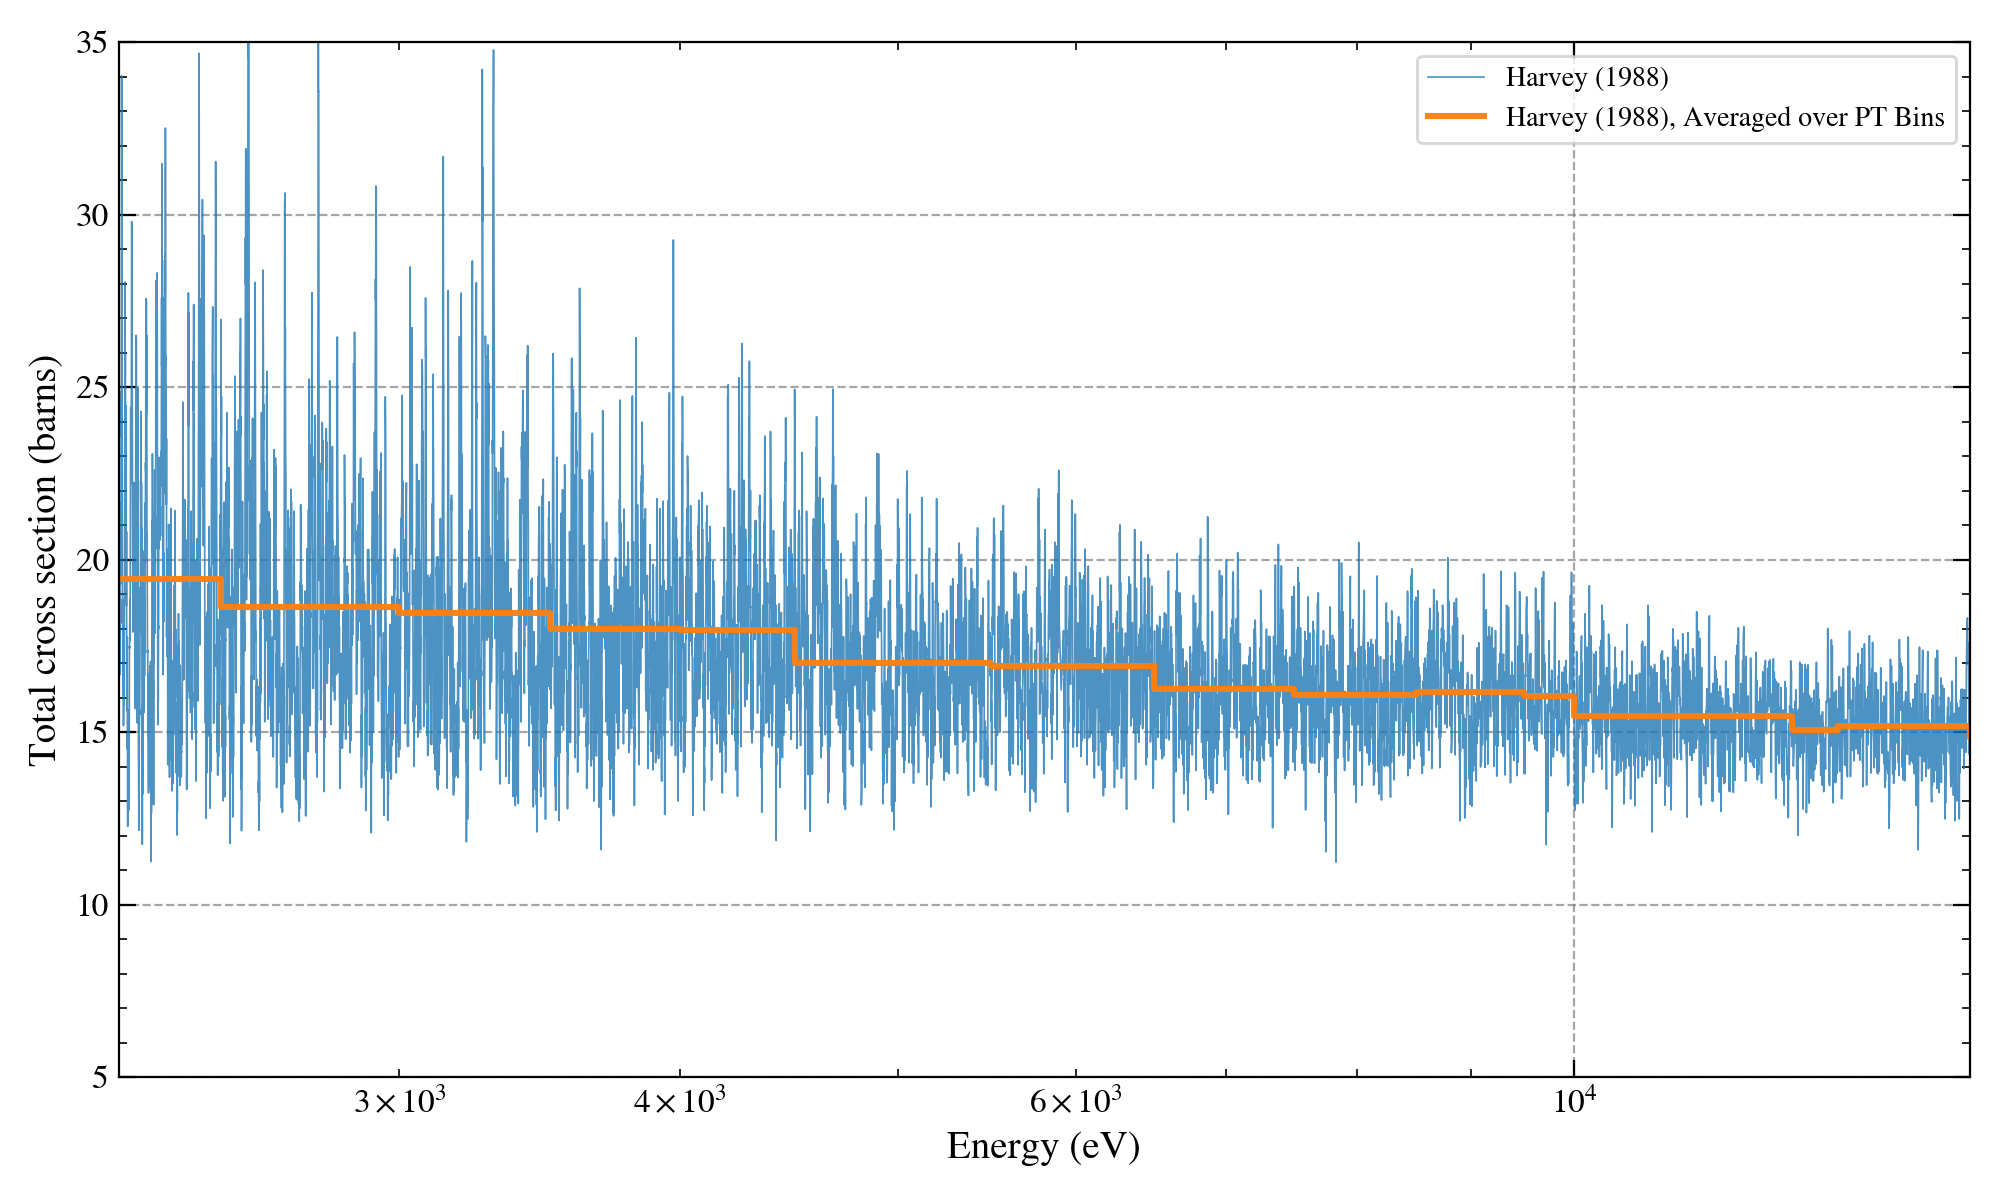
\includegraphics[width=0.95\linewidth]{newfigs/totalxs_comparison.png}\\[0.6em]
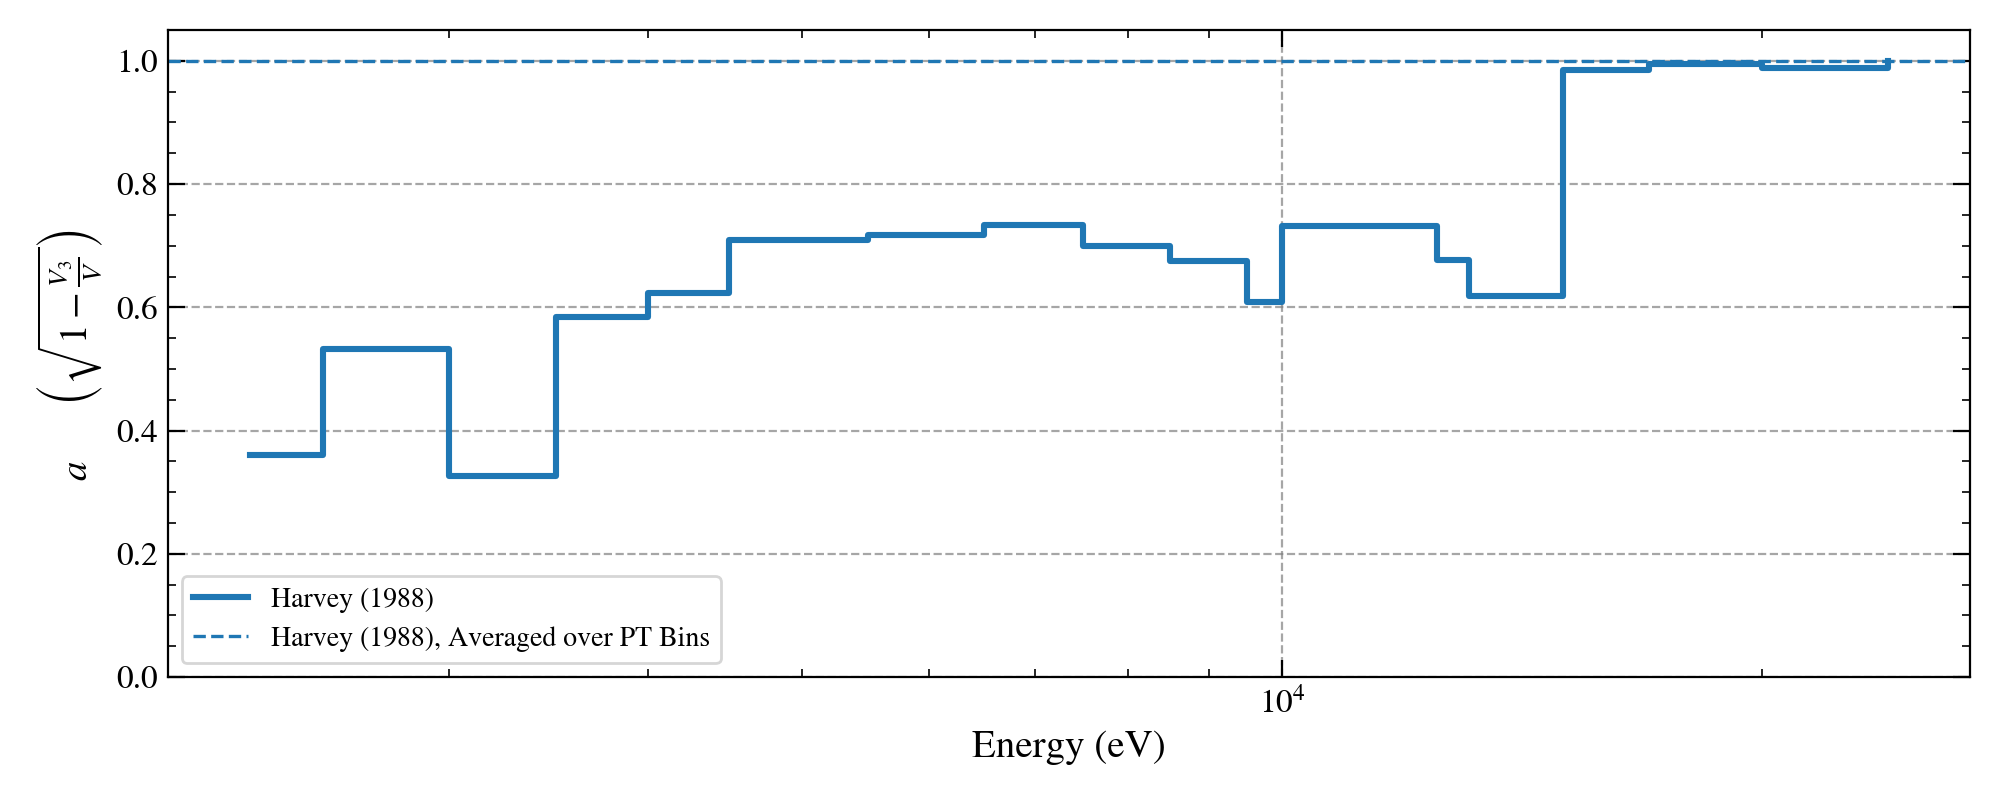
\includegraphics[width=0.95\linewidth]{newfigs/a_param.png}
\caption{Controlled \isotope{235}{U} transmission demonstration inputs. (\textbf{Top}) Pointwise total cross section $\sigma_3(E)$ from the transmission data and its bin-averaged representation $\sbin$ over the probability-table (PURR) energy boundaries. (\textbf{Bottom}) Variance-budget scaling parameter $a(E)=\sqrt{1- V_3/V}$ evaluated in each probability-table bin, where $V_3$ is the within-bin variance of $\sigma_3(E)$ and $V$ is the variance implied by the sampled probability-table distribution in that bin.}
\label{fig:smooth_vs_raw_xs}
\end{figure}

The transmission results are shown in \autoref{fig:comparing-variance-preservation}. The central result is that transferring variance from the probability table to the pointwise File~3 cross section preserves the bin-averaged transmission to within 0.02\%: the variance decomposition of \autoref{eq:var_split} holds at the level of the observable. This is not trivially guaranteed---the decomposition neglects covariance between the File~3 and p-table components, and the transmission is a nonlinear function of the cross section. The success of the decomposition under the deliberately extreme $\sigma_3(E)$ used here provides confidence that it will hold \emph{a fortiori} for the more moderate structure present in the ENDF/B-VIII.1 fission evaluation.

A key outcome of \autoref{fig:comparing-variance-preservation} is that the alternative treatments remain distinctly separated from the reference behavior. The results show a clear ordering: omitting probability tables underestimates self-shielding, while ``double-dipping'' overestimates it. The variance-budgeted treatment is the only case that preserves the reference bin-averaged transmission while still permitting intra-bin modulation from the pointwise $\sigma_3(E)$.

\begin{figure}[htbp]
\centering
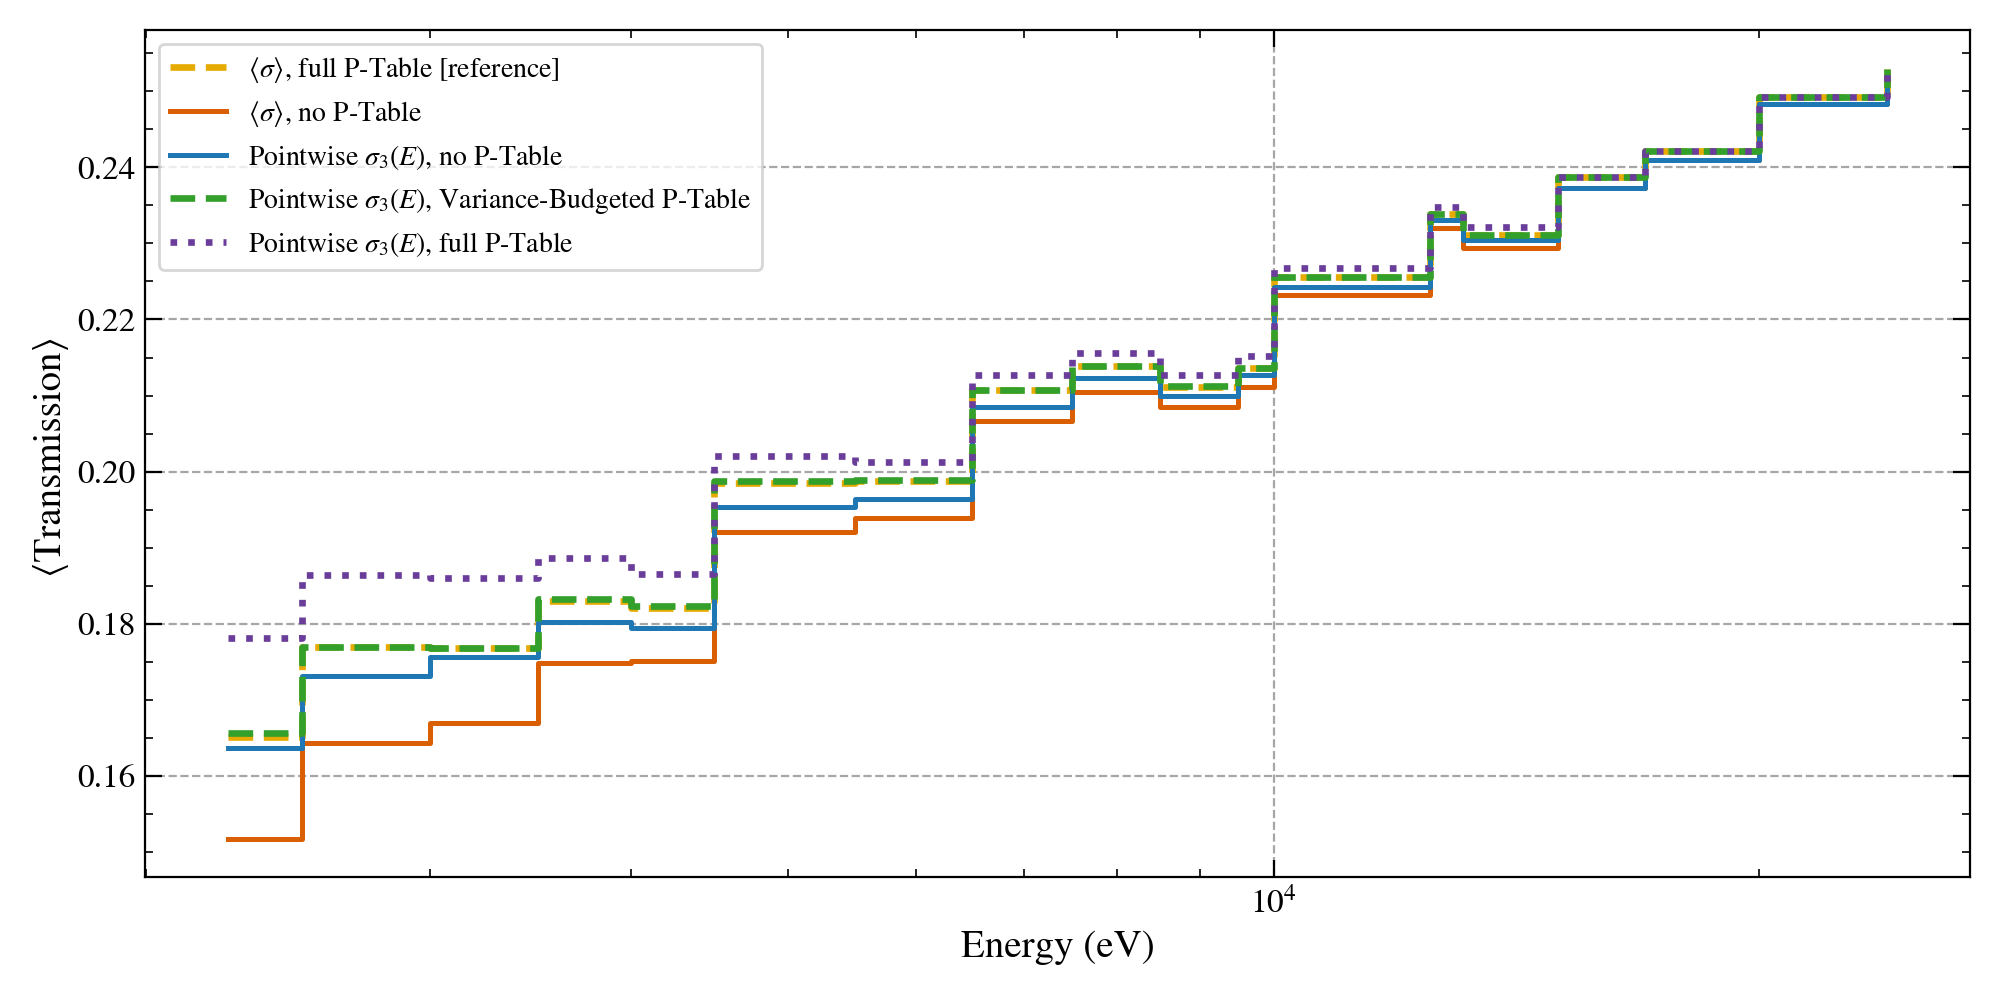
\includegraphics[width=0.95\linewidth]{newfigs/avg_transmissions.png}\\[0.6em]
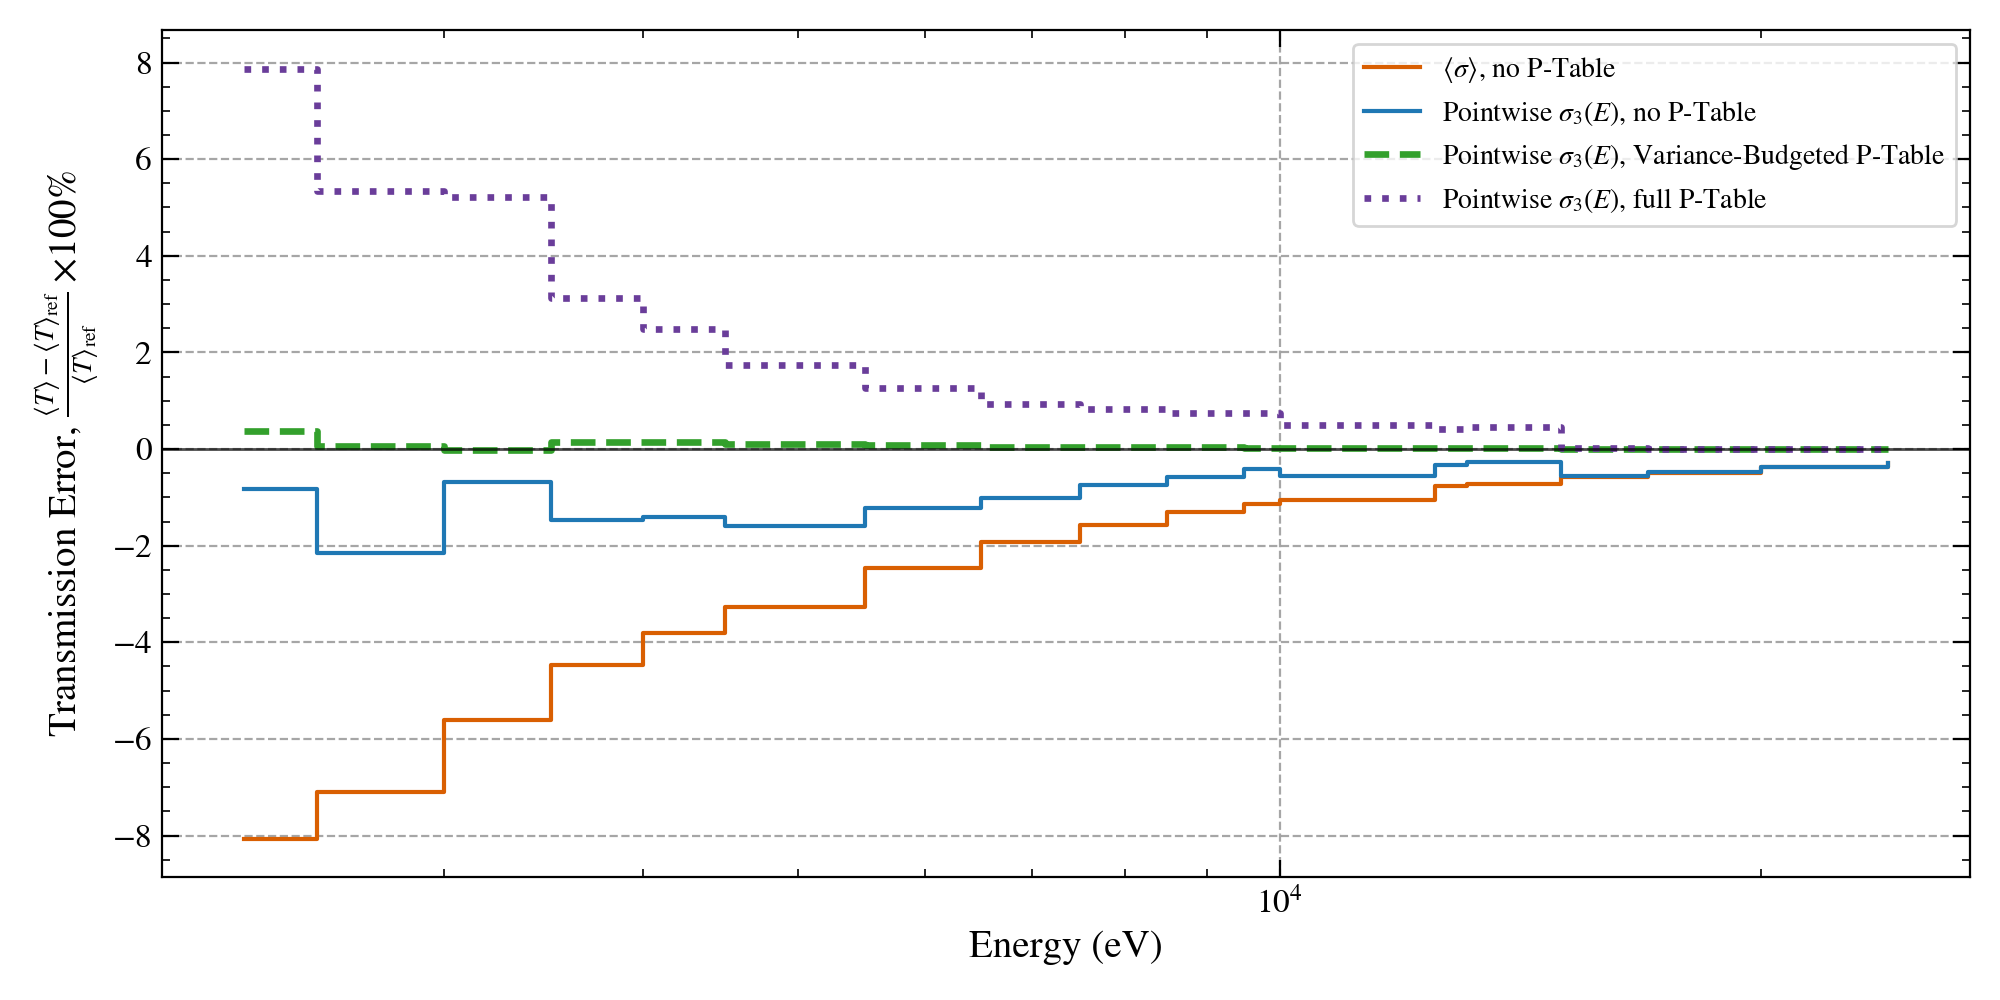
\includegraphics[width=0.95\linewidth]{newfigs/transmission_error.png}
\caption{Transmission comparison for the controlled \isotope{235}{U} test. (\textbf{Top}) Bin-averaged transmissions for five cases: (i) $\sbin$ with no probability-table treatment (un-self-shielded), (ii) $\sbin$ with full probability-table sampling (reference), (iii) raw $\sigma_3(E)$ with no probability-table treatment (semi-self-shielded), (iv) raw $\sigma_3(E)$ with variance-budgeted probability-table sampling, and (v) raw $\sigma_3(E)$ with full probability-table sampling (double-dipping). (\textbf{Bottom}) Transmission ratios relative to the reference case, $T/T_{\mathrm{ref}}$, highlighting the bias introduced by neglecting probability tables or by double counting fluctuations.}
\label{fig:comparing-variance-preservation}
\end{figure}

To quantify this agreement, \autoref{tab:transmission_rms} reports the root-mean-square (RMS), mean bias, and maximum absolute deviation of the binned transmissions relative to the purely probability-table method, which is treated as the reference. Over 2.25--15~keV, the variance-budgeted method reduces the RMS deviation by nearly an order of magnitude compared to using the pointwise File~3 cross section without probability tables, while simultaneously avoiding the large deviations observed for the ``double-dipping'' case.

\begin{table}[h!]
\centering
\caption{Agreement of bin-averaged transmissions in the controlled \isotope{235}{U} demonstration over 2.25--15~keV. The purely probability-table transmission of the bin-averaged cross section ($\sbin$ with full probability-table sampling) is treated as the reference.}
\begin{tabular}{lccc}
\toprule
Method & RMS & Mean bias & Max.\ abs.\ diff. \\
\midrule
$\langle \sigma \rangle$, full P-Table applied [reference] & 0 & 0 & 0 \\
$\langle \sigma \rangle$, no P-Table & 6.109e-03 & -4.719e-03 & 1.332e-02 \\
Pointwise $\sigma_3(E)$, no P-Table & 1.884e-03 & -1.660e-03 & 3.805e-03 \\
Pointwise $\sigma_3(E)$, Variance-Budgeted P-Table & 1.859e-04 & 1.109e-04 & 6.165e-04 \\
Pointwise $\sigma_3(E)$, full P-Table & 4.882e-03 & 3.224e-03 & 1.298e-02 \\
\bottomrule
\end{tabular}
\label{tab:transmission_rms}
\end{table}

%-----------------------------------------------------------------------------
\subsection{Per-Reaction Variance Budget for \isotope{235}{U}}
\label{ssec:per-reaction-results}
%-----------------------------------------------------------------------------

With the variance decomposition validated, the per-reaction implementation (\autoref{sssec:per-reaction-a}) is applied to the \isotope{235}{U} evaluations. \autoref{fig:v3-total}--\autoref{fig:v3-elastic-capture} show the within-bin File~3 variance $V_{3,r}$ for all four reaction channels at each PURR grid point, comparing ENDF/B-VIII.0 and VIII.1 (the fission channel was shown previously in \autoref{fig:v3-fission}). The dominant change between evaluations is concentrated in the fission channel: $V_{3,\text{fis}}$ increases by roughly an order of magnitude across most of the URR. The total cross section inherits this increase because $\sigma_{\text{tot}} = \sigma_{\text{el}} + \sigma_{\text{fis}} + \sigma_{\text{cap}}$ and the fission variance dominates. By contrast, the elastic and capture channels show essentially no change between evaluations, with $V_{3,\text{el}}$ and $V_{3,\text{cap}}$ remaining two to three orders of magnitude below the fission variance.

\begin{figure}[htbp]
\centering
%\includegraphics[width=0.95\linewidth]{figures/fig_v3_total.pdf}
\caption{Within-bin File~3 variance $V_{3}$ for the total cross section at each PURR energy grid point. ENDF/B-VIII.0 (squares) and VIII.1 (circles) are compared. The increase in VIII.1 is inherited entirely from the fission channel.}
\label{fig:v3-total}
\end{figure}

\begin{figure}[htbp]
\centering
%\includegraphics[width=0.48\linewidth]{figures/fig_v3_elastic.pdf}\hfill
%\includegraphics[width=0.48\linewidth]{figures/fig_v3_capture.pdf}
\caption{Within-bin File~3 variance for the elastic (left) and capture (right) channels. Both are negligible ($V_3 \lesssim 10^{-2}$~b$^2$) and essentially unchanged between evaluations.}
\label{fig:v3-elastic-capture}
\end{figure}

To determine the variance-budgeting parameter $a_r$ at each grid point, the File~3 variance $V_{3,r}$ must be compared against the sampled probability-table variance $V_r$ from PURR. \autoref{fig:u235-variance-budget} shows the effective transport variance for the fission cross section under three processing scenarios: ENDF/B-VIII.0 with standard \texttt{LSSF=1} (baseline), ENDF/B-VIII.1 with standard \texttt{LSSF=1} (double counting), and ENDF/B-VIII.1 with per-reaction variance budgeting (corrected). In the standard VIII.1 processing, the transport sees a total fission variance of $V_{3,\text{fis}} + V_{\text{fis}}$ (File~3 structure plus full p-table modulation), which exceeds the intended compound-nucleus fluctuation variance $V_{\text{fis}}$. The variance-budgeted processing reduces the p-table contribution to the residual $V_{\text{fis}} - V_{3,\text{fis}}$, restoring the total effective variance to $V_{\text{fis}}$.

\begin{figure}[htbp]
\centering
%\includegraphics[width=0.95\linewidth]{figures/u235_fission_variance_comparison.pdf}
\fbox{\parbox{0.9\linewidth}{\centering\vspace{3em}\textbf{Placeholder:} Effective transport variance of the \isotope{235}{U} fission cross section vs.\ energy for three cases: ENDF/B-VIII.0 (\texttt{LSSF=1}), ENDF/B-VIII.1 (\texttt{LSSF=1}, double counting), and ENDF/B-VIII.1 (variance-budgeted). Requires PURR sampled variance $V_{\text{fis}}$ from ladder sampling.\vspace{3em}}}
\caption{Effective transport variance of the \isotope{235}{U} fission cross section across the URR. ENDF/B-VIII.0 with standard processing serves as the baseline (File~3 variance small, p-table carries most of $V$). Standard VIII.1 processing shows inflated variance from double counting. Variance-budgeted VIII.1 processing restores the intended total fluctuation variance by reducing the p-table contribution.}
\label{fig:u235-variance-budget}
\end{figure}

\begin{figure}[htbp]
\centering
%\includegraphics[width=0.95\linewidth]{figures/u235_a_param_per_reaction.pdf}
\fbox{\parbox{0.9\linewidth}{\centering\vspace{3em}\textbf{Placeholder:} Per-reaction variance-budgeting parameter $a_r(E)$ for the ENDF/B-VIII.1 \isotope{235}{U} evaluation. Requires PURR sampled variance $V_r$ to compute $a_r = \sqrt{1 - V_{3,r}/V_r}$. Expected: $a_{\text{el}} \approx a_{\text{cap}} \approx 1$ (smooth), $a_{\text{fis}} < 1$ (structured), $a_{\text{tot}}$ intermediate.\vspace{3em}}}
\caption{Per-reaction variance-budgeting parameter $a_r$ for \isotope{235}{U} (ENDF/B-VIII.1) at each PURR energy grid point. The elastic and capture channels have negligible File~3 variance ($a \approx 1$), while the fission channel shows $a_{\text{fis}} < 1$ where File~3 structure carries a significant fraction of the total fluctuation variance. The total cross section inherits a reduced $a$ from the fission contribution.}
\label{fig:a-per-reaction}
\end{figure}

The per-reaction nature of the variance budget is critical. Although the total cross section also shows increased $V_3$ in VIII.1, this is entirely inherited from the fission channel. Computing $V_3$ and $a$ independently for each reaction channel correctly identifies the fission partial as the source of the double-counting problem and applies the appropriate correction without affecting the elastic or capture channels.

%-----------------------------------------------------------------------------
\subsection{Critical Benchmark Results}
\label{ssec:crit-benchmark-results}
%-----------------------------------------------------------------------------

Integral transport calculations are performed with \textsc{MCNP}~6.3 \cite{mcnp}. The selected benchmark is HEU-MET-INTER-011 \cite{icsbep,mcurie}, a highly enriched \isotope{235}{U} metal sphere with intermediate-spectrum leakage (a configuration designed to be sensitive to URR self-shielding treatments). In each case, the ACE-format cross sections are generated with NJOY \cite{njoy}. All other isotopes in the problem are left unchanged between runs so that differences in reactivity can be attributed directly to the \isotope{235}{U} treatment.

\autoref{tab:consolidated_benchmark} reports the HEU-MET-INTERM-011 benchmark calculations for four \isotope{235}{U} URR treatments: ENDF/B-VIII.0 with standard \texttt{LSSF=1} processing, ENDF/B-VIII.1 with standard \texttt{LSSF=1}, ENDF/B-VIII.1 with variance-preserved processing (mean-shift correction, $a=1$), and probability tables disabled entirely (P-Tables OFF). All statistical uncertainties are $\pm 0.00002$ in $k_{\text{eff}}$.

\begin{table}[!t]
\centering
\caption{Consolidated $k_{\text{eff}}$ results for HEU-MET-INTERM-011. Four \isotope{235}{U} URR treatments are compared. $\Delta\rho_{\text{VP}}$ is the reactivity shift from variance preservation relative to VIII.1 (standard); $\Delta\rho_{\text{SS}}$ is the total URR self-shielding worth (P-Tables OFF minus VIII.1 standard). Fraction gives $\Delta\rho_{\text{VP}}/\Delta\rho_{\text{SS}}$. All $k_{\text{eff}}$ uncertainties are $\pm 0.00002$.}
\begin{tabular}{lcccccccc}
\toprule
Case & VIII.0 & VIII.1 & VIII.1 & P-Tables & $\Delta\rho_{\text{VP}}$ & $\Delta\rho_{\text{SS}}$ & Fraction \\
& (LSSF=1) & (LSSF=1) & (Var-Pres) & OFF & (pcm) & (pcm) & \\
\midrule
1 & \textit{TBD} & 1.00752 & 1.00765 & 1.00829 & $+13$ & $+76$ & 17\% \\
2 & \textit{TBD} & 1.00663 & 1.00679 & 1.00749 & $+16$ & $+85$ & 19\% \\
3 & \textit{TBD} & 1.00541 & 1.00555 & 1.00631 & $+14$ & $+89$ & 16\% \\
4 & \textit{TBD} & 1.00495 & 1.00510 & 1.00584 & $+15$ & $+88$ & 17\% \\
5 & \textit{TBD} & 1.00242 & 1.00255 & 1.00335 & $+13$ & $+92$ & 14\% \\
\bottomrule
\end{tabular}
\label{tab:consolidated_benchmark}
\end{table}

Across the five cases, the variance-preserving treatment yields a consistent positive reactivity shift of 13--16~pcm (mean $\sim$14~pcm) relative to the standard VIII.1 method, corresponding to approximately 16\% of the total URR self-shielding reactivity worth (76--92~pcm). The positive sign is consistent with the expectation that the standard method over-predicts self-shielding via inflated variance, so that correcting the variance produces a net positive reactivity shift.

Because the only change between the standard and variance-preserved cases is the \isotope{235}{U} probability-table scaling procedure, the consistent sign and magnitude of the shift across the five cases---which span a range of sphere radii and hence spectral hardness---supports the interpretation that the effect is systematic rather than configuration-specific.

The VIII.0 column will enable isolation of the reactivity bias attributable to fission-channel variance double counting once those calculations are complete. The difference between VIII.1 (variance-preserved) and VIII.0 will reflect the physics-only evaluation change, with the double-counting artifact removed.

%=============================================================================
\section{Discussion}
\label{sec:discussion}
%=============================================================================

%-----------------------------------------------------------------------------
\subsection{Transmission Test Residuals}
%-----------------------------------------------------------------------------

\autoref{fig:comparing-variance-preservation} shows the relative transmission error of several self-shielding treatments with respect to the reference transmission case (smooth cross-section, variance entirely defined by probability tables). As expected, the variance-budgeted treatment applied to the pointwise cross section reproduces the reference transmission to within a small fraction of a percent across nearly the entire unresolved resonance range.

An exception occurs in the first unresolved energy bin, where the variance-budgeted result exhibits a small but systematic deviation from the reference transmission. This behavior is not unexpected. The first unresolved resonance bin is inherently the least statistical region of the URR: it is closest to the RRR/URR transition, is most sensitive to bin-edge choices and incomplete resonance population within the bin, and is therefore where any mismatch between a coarse probability-table representation and a deliberately aggressive pointwise $\sigma_3(E)$ is most likely to appear.

It should also be taken into consideration that the pointwise $\sigma_3(E)$ used in \autoref{fig:comparing-variance-preservation} is a deliberately aggressive test constructed directly from reported cross-sections, with no additional processing. Raw experimental cross sections inevitably contain statistical counting noise and residual systematic effects. As a result, the apparent within-bin variance of the pointwise series can exceed the physically meaningful fluctuation content that the URR statistical model is intended to represent. This matters because the variance-budgeting factor, as given in \autoref{eq:a_def}, would return as an imaginary value if $V_3 > V$ which is nonphysical. Nevertheless, even under this deliberately pathological input, the variance-budgeted treatment reduces the RMS transmission error by nearly an order of magnitude relative to all other methods (\autoref{tab:transmission_rms}), confirming that the approach remains robust well beyond the regime of practical interest.

Another argument against using highly structured data in the URR is due to limitations from current processing codes. As of now, industry standard processing workflows do not perform full Doppler broadening of unresolved-range pointwise structure. Only the probability tables themselves would receive temperature dependent treatment in the URR, which could lead to numerical issues.\cite{Cullen2012ENDF370,TrellueLittle2008ENDF70Processing} Consequently, highly resonant structure would not transfer well to other temperatures, and would only be representative of temperatures representative of the experimental conditions of the particular measurement.

%-----------------------------------------------------------------------------
\subsection{Motivations for Structured URR Representations}
%-----------------------------------------------------------------------------

All this being said, there are still motivations behind having a highly structured URR, namely in mixtures. Strong resonances in one isotope can depress the flux across an energy neighborhood and reduce the visibility of smaller resonances in other isotopes (a \emph{resonance shadow}\cite{Carlvik1967Dancoff}), while energy neighborhoods without large resonances allow smaller features to be comparatively more prominent (a \emph{resonance window}\cite{Furuta1987WindowEffect}). This ``window/shadow'' language is a natural way to describe the same nonlinearity that motivates probability tables in the first place. Transmission (and reaction rates) depend on the statistics of $\sigma(E)$, not only on the bin mean \cite{Descalle2023URRPT}.

Independent probability-table sampling erases that coupling. While probability tables correctly sample the single-isotope infinitely-dilute distribution, the transport calculation applies these samples in the presence of other isotopes. Independent sampling at each collision discards energy-correlated structure that, if retained in File~3, would allow the transport solver to capture resonance-overlap effects between isotopes within a mixture. This motivates retaining some physically meaningful energy dependence in the smooth component used during transport (conceptually the File~3 ``mean''), while letting the probability table represent only the remaining unresolved fluctuation variance. In the language of \autoref{ssec:double-dipping}, this is naturally phrased as a variance budget: allow the smooth component to carry mixture-relevant structure (windows and shadows) while the probability-table component carries the compound-nucleus variance needed for self-shielding. The variance-budgeting affine transform derived in this paper provides a controllable way to do that without double counting.

%-----------------------------------------------------------------------------
\subsection{Role of Average Resonance Parameters in Probability Table Variance}
\label{ssec:file2-compound-nucleus}
%-----------------------------------------------------------------------------

The motivation for treating URR probability tables as \emph{compound-nucleus statistics} is primarily
pragmatic: it cleanly separates the role of unresolved fluctuations from the many additional modeling
choices that influence the mean cross section. In modern URR practice, evaluators may introduce
supplementary smooth ``knobs'' (e.g., distant level parameters, background terms, or model-specific
mean adjustments) to reproduce integral data and match target infinite-dilute cross sections.
These quantities can be important for the mean behavior, but they are not the object that probability
tables were designed to encode.

Probability tables are a discrete representation of a \emph{fluctuation distribution} generated from statistical assumptions of average resonance parameters. For self-shielding, the essential requirement is not that every contributor to the mean be represented within the same file, but that the transport code receives a distribution with the correct mean \emph{and} the correct fluctuation variance. This observation motivates a division of labor: the smooth mean cross section may include any evaluator-chosen structure or background adjustments, while the probability table should be interpreted as the compound-nucleus fluctuation content that controls URR variance.

This division of labor has a practical advantage: the proposed variance-preserving correction does not require any changes to the evaluator's URR model choices or to how additional smooth parameters are encoded. Existing probability tables may be retained exactly as generated; only the \emph{mean-enforcement} step is modified to avoid nonphysical variance scaling when the sampled table mean differs from the evaluator's bin-averaged mean.

%-----------------------------------------------------------------------------
\subsection{Backwards Compatibility}
\label{ssec:backwards-compat}
%-----------------------------------------------------------------------------

A practical concern is that many evaluations and processed libraries have been produced, validated, and in some cases benchmark-tuned under the historical \texttt{LSSF=1} workflow. Retroactively changing the interpretation of \texttt{LSSF=1} probability tables risks perturbing established performance---including cases where compensating effects may have been implicitly absorbed during evaluation or validation.

The fact that this systematic error has not been widely identified in past URR evaluations is consistent with how probability tables are typically deployed in production libraries and processing. If $V_3\approx 0$, then $a\to 1$ and \autoref{eq:sigma_prime_budget} reduces to the pure mean shift in \autoref{eq:affine_shift}--\autoref{eq:Delta_def}. If additionally $\sbin=\mu$, then $f'_j=\sigma_j/\mu$, recovering the original factor definition (\autoref{eq:ptable-orig-factor}). These limiting cases also explain why variance-scaling pathologies have been easy to miss in practice: many production evaluations and processing chains operate close to $V_3\approx 0$ and $\sbin\approx\mu$, so the \texttt{LSSF=1} factor method behaves as intended. In particular, \texttt{LSSF=1} is motivated not only to enforce the evaluator's infinitely-dilute mean when $\mu\neq\sbin$, but also to reduce the sampling burden by decoupling the reported mean from statistical noise in finite sampling \cite{endf-manual}. In that usage, the resulting bias is insignificant. The issue arises when the same multiplicative enforcement is effectively used to scale the cross-section distribution itself, which rescales the fluctuation variance whenever $\sbin/\mu\not\approx 1$.

However, the ENDF/B-VIII.1 \isotope{235}{U} evaluation (\autoref{sssec:u235-evaluation-change}) represents a case where the standard workflow breaks down: the fission File~3 carries substantial within-bin variance ($V_{3,\text{fis}}$ up to $\sim$2.5~b$^2$), but the probability table is unmodified, producing measurable variance double counting. As shown in \autoref{ssec:crit-benchmark-results}, even the mean-enforcement correction alone (with $a = 1$) produces a $\sim$14~pcm positive reactivity shift, and the per-reaction variance budget (\autoref{ssec:per-reaction-results}) addresses the additional fission-channel double counting. Retroactively applying these corrections to an evaluation that may have been tuned under the standard method could degrade benchmark agreement without corresponding improvement in the underlying physics.

For this reason, the variance-preserving affine transformations derived in \autoref{sec:theory} should be treated as a forward-looking option rather than a retroactive reinterpretation. A straightforward implementation path is to introduce a new switch (e.g., \texttt{LSSF=2}) that explicitly requests variance-preserving reconstruction, while keeping \texttt{LSSF=1} behavior unchanged for legacy data. This enables new evaluations and reprocessed libraries to opt into variance preservation in a traceable and reviewable way, without silently altering the semantics of existing libraries. The broader importance of unambiguous processing/transport interpretation and the limits imposed by the ENDF-6 format are recurring themes in the URR community discussions \cite{wpec32,endf-manual}.

%=============================================================================
\section{Conclusions}
%=============================================================================

Probability tables remain a practical technique for representing URR self-shielding effects in Monte Carlo neutron transport. However, to maintain physical fidelity, they must preserve the variance implied by the sampled resonance physics. This paper has identified two mechanisms by which standard processing can distort that variance---multiplicative mean enforcement and File~3 variance double counting---and derived a unified affine-transformation framework that addresses both.

The common practice of enforcing mean consistency via multiplicative renormalization can inadvertently rescale the distribution and bias self-shielding. A variance-preserving correction follows naturally: enforce the evaluator mean via an additive shift (or, when retaining within-bin structure, a variance-budgeted affine transform) without altering the intended unresolved variance.

This issue has become practically relevant with the ENDF/B-VIII.1 evaluation of \isotope{235}{U}, which introduced substantial fission cross-section structure in the URR derived from the Weston \& Todd~\cite{WestonTodd1992} measurement. Under standard processing, this structure creates variance double counting in the fission channel. The per-reaction variance-budgeting methodology developed here, and implemented in the PURR module of NJOY (\autoref{ssec:njoy-implementation}), addresses this problem by computing the File~3 variance $V_{3,r}$ independently for each reaction and reducing the probability-table modulation accordingly---all within the existing \texttt{LSSF=1} factor format, requiring no changes to transport codes.

Through controlled transmission tests, the variance decomposition has been validated under a deliberately extreme test case. Integral benchmark calculations demonstrate that even the mean-enforcement correction alone produces a measurable $\sim$14~pcm reactivity shift in the HEU-MET-INTERM-011 benchmark suite, corresponding to approximately 16\% of the total URR self-shielding worth.

\subsection{Future Work}
\begin{itemize}
\item Completion of the ENDF/B-VIII.0 vs.\ VIII.1 benchmark comparison with per-reaction variance budgeting to isolate the reactivity impact of fission-channel double counting.
\item Extension of the implementation to additional isotopes and evaluations with significant File~3 structure in the URR.
\item Further study of the limits of neglecting covariance between the retained pointwise structure and the unresolved fluctuation component.
\end{itemize}

\bibliographystyle{style/ans_js}
\bibliography{bibliography}

\end{document}
